\chapter{The SpiNNaker Architecture}
	
	\label{sec:background}
	
	The Spiking Neural Network Architecture (SpiNNaker) is a massively parallel
	computer architecture designed to simulate biologically realistic neural
	models \cite{furber07}. In this chapter we will explore this unconventional
	architecture in detail, starting with its purpose and then focusing on its
	network.
	
	% * Purpose
	%   * Spiking neural simulations
	%     * Neural modelling: PyNN, Nengo...
	%     * Parallelisation + communication
	
	\section{Neural simulation}
		
		Human brains contain billions of \emph{neurons} connected together by
		trillions of \emph{synapses}. The neurons communicate by transmitting and
		receiving \emph{spikes} through their synapses. Each spike is `valueless'
		in that a spike's only significant features are when it is received and
		which neuron it came from.
		
		\begin{figure}
			\center
			\buildfig{figures/lif-neuron.tex}
			
			\caption{A Leaky Integrate-and-Fire (LIF) neuron.}
			\label{fig:lif-neuron}
		\end{figure}
		
		Though very detailed models of the electrochemical processes occurring
		inside neurons are computationally intensive, simplified models such as the
		Leaky Integrate-and-Fire (LIF) model can be implemented in just a handful
		of CPU instructions\footnote{Or, in the case of figure~\ref{fig:lif-neuron},
		seven lines of \LaTeX{}.} \cite{vainbrand11}. Figure~\ref{fig:lif-neuron}
		illustrates a simple LIF neuron in which incoming spikes cause charge to
		build up (integrated). Over time this charge leaks away but if an incoming
		spike causes the charge to rise above a certain threshold, the neuron
		`fires' producing a spike. Despite the simplicity of this model, large
		neural networks such as Spaun \cite{eliasmith12}, built entirely from LIF
		neurons, exhibit complex behaviours such as fine motor control and problem
		solving.
		
		The computational expense of large scale neural simulations arises not from
		modelling the neurons but distributing the spikes they produce. In biology,
		neurons produce spikes at an average rate of \SI{10}{\hertz} and synapses
		connect each neuron's output to (order) \num{1000} neurons
		\cite{navaridas09}. In a neural model with, for example, \num{70000000}
		neurons (approximately the number in a house mouse), this rate of spike
		production equates to \num{700000000} spikes produced per second.  Because
		each spike is sent to many neurons, this equates to \num{700000000000}
		spikes being received per second. If each spike is transmitted as a single
		UDP datagram in a conventional computer network, assuming the spike could
		be encoded as a \SI{32}{\bit} value, this corresponds with a total network
		throughput of \SI{179.2}{\tera\bit\per\second}. At the time of writing,
		this is more than double the bisection bandwidth (theoretical worst case
		throughput) of the world's most powerful super computer \cite{dongarra16}.
	
	\section{Network architecture}
		
		Architectures such as IBM's Blue Gene \cite{chiu11} and Cray's XK7
		\cite{ornl16} employ powerful compute nodes connected together using
		networks designed to transfer of chunks of kilobytes of data between nodes.
		Since neural models have relatively light computational requirements and
		communications are based on very small pieces of data (spikes), this type
		of architecture is poorly suited to the task.
		
		SpiNNaker's architectural target is to support realtime simulations of up
		to one billion neurons. Since neural models such as LIF are inexpensive to
		model and many neurons can be simulated independently in parallel,
		SpiNNaker employs many small, energy efficient ARM processors
		\cite{furber07}. To support the unusual communication requirements of
		neural simulations, SpiNNaker employs a bespoke interconnection network.
		
	%   * SpiNNaker chip
	%     * Cores
	%     * SDRAM
	%     * NoC
	%     * Router
		
		\begin{figure}
			\center
			%
\includegraphics[width=19mm]{figures/spinnakerChip.jpg}
			\buildfig{figures/hex-chips.tex}
			
			\caption{SpiNNaker chips (actual size) connected to their six neighbours.}
			\label{fig:spinnakerChip}
		\end{figure}
		
		The fundamental building block of the SpiNNaker architecture is the
		SpiNNaker chip (figure \ref{fig:spinnakerChip}) \cite{furber13}. Each chip
		contains eighteen low power ARM 968 processor cores each capable of
		simulating between \num{200} and \num{2000} LIF neurons in real time
		\cite{mundy15}.  Each core has a total of \SI{96}{\kilo\byte} of private
		Tightly-Coupled Memory (TCM) and shares access to \SI{128}{\mega\byte} of
		on-chip SDRAM with other cores on the same chip. Finally, each chip
		contains a programmable router which routes network packets to and from the
		local cores and six neighbouring SpiNNaker chips. SpiNNaker machines are
		constructed by combining many SpiNNaker chips.
		
		\begin{figure}
			\center
			\buildfig{figures/spinnaker-packet.tex}
			
			\caption{SpiNNaker's \SI{40}{\bit} and \SI{72}{\bit} multicast packet
			format.}
			\label{fig:spinnaker-packet}
		\end{figure}
		
		Processor cores can communicate by sending and receiving network packets
		forwarded by routers through the network. Since SpiNNaker's network is
		designed to efficiently transmit neural spike events, individual network
		packets are small, either \SI{40}{\bit} or \SI{72}{\bit} compared with tens
		or hundreds of bytes in typical network architectures.
		
		In a spiking neural simulation, the only significant features of a spike is
		its the identity of the neuron which produced it and the time it was
		produced. In a real-time simulation, the time at which a spike is produced
		is implicitly indicated by the time at which the spike is received since at
		biological timescales a computer network delivers packets
		`instantaneously'. Consequently, the only data which must be explicitly
		encoded is the identity of the neuron which produced the spike. In
		SpiNNaker, a spike may be encoded by using a single \SI{40}{\bit}
		`multicast packet' whose format is illustrated in
		figure~\ref{fig:spinnaker-packet}.  The \SI{8}{\bit} header is used by
		SpiNNaker's routers to determine the type of packet and the \SI{32}{\bit}
		`routing key' is used to uniquely identify the neuron which produced the
		packet. This neuron identifier is also used by SpiNNaker's router to
		determine how the packet should be routed through the network. The optional
		\SI{32}{\bit} payload is not used by conventional spiking neural
		simulations.
	
	\section{The SpiNNaker router}
		
		The SpiNNaker router employs an unconventional design which, despite its
		compact size and low energy requirements, implements a flexible multicast
		routing scheme. Unlike conventional routers which often employ hard-coded
		routing rules \cite{dally04}, the SpiNNaker router uses a programmable
		`routing table' to determine how packets should be forwarded.
		
		In addition, to avoid deadlocks SpiNNaker's router employs a simple
		timeout-based mechanism which exploits the ability of neural networks to
		tolerate occasional missing packets. As we will see in chapter
		\ref{sec:routing}, this timeout-based mechanism greatly simplifies the task
		of routing in SpiNNaker's network.
		
		In this section we'll see how each of these distinctive features of
		SpiNNaker's router are used.
		
		\subsection{Routing tables}
		
			When a multicast packet arrives at a SpiNNaker router (either from a
			local core or neighbouring chip), the router looks up the routing key in
			its routing table. This table consists of \num{1024} table entries, each
			of which specifies a routing key bit pattern to match and a set of
			routes.  When a multicast packet's routing key matches a routing entry
			the packet is forwarded along every route specified in the entry,
			potentially duplicating the packet. This technique allows packets to be
			transmitted once but received in a number of places while making
			efficient use of the network \cite{navaridas12}.  Though routing table
			entries are very limited in supply (with only \num{1024} entries per
			router), complex routing patterns with many thousands of traffic flows
			can be routed by a single router. The bit pattern within each routing
			entry may match against the bits of a routing key as either `\texttt{1}',
			`\texttt{0}' or `\texttt{X}' (don't care). This means that a single
			routing entry may, for example, be used to match routing keys with a
			certain prefix. In addition, if a routing key is not matched by any entry
			in the routing table then the packet is `default routed' in a straight
			line. For example if a packet arrived from the chip to the left, the
			packet will be default routed to the chip on the right. By assigning
			routing keys such that neurons whose spikes are sent to similar
			destinations share a similar prefix, the number of routing entries
			required by a simulation is greatly reduced \cite{davies12}.
			
			\begin{figure}
				\center
				\buildfig{figures/routing-example.tex}
				
				\caption{Multicast routing example with \SI{4}{\bit} routing keys.}
				\label{fig:routing-example}
			\end{figure}
			
			Consider the example figure~\ref{fig:routing-example} in which
			\SI{4}{\bit} routing keys are used by packets and a number of routing
			table entries have been configured. If a packet with the routing key
			\texttt{1011} is transmitted by a core in chip $(0, 0, 0)$, this will
			match the first routing table entry on that chip and will be routed to
			chip $(1, 0, 0)$. On chip $(1, 0, 0)$, the packet once again matches the
			first routing entry and is routed to chip $(1, 0 -1)$. On $(1, 0 -1)$,
			however, the packet does not match the routing table entry on that chip
			and so is default routed to $(1, 0, -2)$. At this chip, the packet
			matches a routing entry which routes the packet to core~7. Here default
			routing allows only three routing table entries to direct a packet
			through four chips.
			
			As a second example, if a packet with the routing key \texttt{0010} is
			transmitted by a core on chip $(0, 0, 0)$, this key will be matched by
			the second routing entry since \texttt{X}s in the table entry will match
			both \texttt{1}s and \texttt{0}s in a routing key. When the packet
			arrives at chip $(0, 0, -1)$ the matching routing entry forwards the
			packet to both $(0, 1, -1)$ and $(1, 0, -1)$ simultaneously. The copy of
			the packet arriving at $(0, 1, -1)$ is immediately routed to core~5 on
			that chip.  Meanwhile, the copy forwarded to $(1, 0, -1)$ is duplicated
			again with one copy being routed to core~11 and another being routed to
			chip $(1, 0, -2)$ where the packet is finally delivered to core~6. In
			this example, the ability of the router to multicast (duplicate) packets
			as they pass through the network meant that sending one copy of the
			packet was sufficient to reach three destination cores. In addition, by
			using \texttt{X}s in the routing table entry, the same routing entries
			are sufficient to route packets with the any of the keys \texttt{0000},
			\texttt{0001}, \texttt{0010} and \texttt{0011}.
		
		\subsection{Timeouts}
			
			\begin{figure}
				\center
				\buildfig{figures/router-architecture.tex}
				
				\caption{SpiNNaker router architecture}
				\label{fig:router-architecture}
			\end{figure}
			
			SpiNNaker's router is built on a pipeline architecture. As shown in
			figure~\ref{fig:router-architecture}, the router is fed packets by an
			arbiter which serialises packets arriving from other chips and local
			cores. Every (\SI{100}{\mega\hertz}) clock cycle, the router routes a
			single packet to one or several output links. If any output port the
			packet is to be routed to is busy then the packet is not forwarded to any
			output link and the router stalls. Once a packet is blocked for a
			programmable number of cycles, it is dropped (discarded). Links become
			busy while transmitting packets or waiting for the receiver to become
			ready. For example, a receiving processor core may be busy performing
			some computation or a receiving router may be blocked waiting for some if
			its outputs to become ready.
			
			This timeout-based packet dropping mechanism is designed to defuse
			deadlocks in the network. For example, if two routers are trying to send
			each other a packet at the same time they may become deadlocked, each
			waiting for the other router to accept the packet they're sending before
			processing any other packets. SpiNNaker's timeout mechanism breaks this
			type of deadlock by dropping the packets after they have been blocked for
			a some time. Once a packet has been dropped it is usually left to the
			software to either tolerate the missing packet or trigger a
			retransmission. In neural simulations, as in biology, the loss of a
			single spike is unlikely to have a significant impact on the behaviour of
			a neural model and therefore neural simulations are inherently tolerant
			of occasional dropped packets. During application loading and other
			system tasks, a higher level software driven protocol based on
			acknowledgements and retransmissions is used to ensure guaranteed
			delivery.
			
			% TODO: MENTION TIMEOUT VALUE USED?
			% Router timeouts must be configured to be long enough that delays in
			% packet transmission, for example due to the time taken for packets to
			% traverse a link, do not trigger packet dropping. Conversely, the timeout
			% should be as short as possible in order to reduce the time the router is
			% blocked and maximise network throughput.
	
	\section{The hexagonal torus topology}
		
		\begin{figure}
			\center
			\buildfig{figures/hexagonalTorusTopology.tex}
			
			\caption{A hexagonal torus topology. Each hexagon represents a
			SpiNNaker chip. Touching chips are directly connected. Chips on edges
			$a$, $b$ and $c$ are also directly connected to the corresponding chips
			on edges $a'$, $b'$ and $c'$, respectively. The three axes of the
			topology, `X', `Y' and `Z' are also shown.}
			\label{fig:hexagonalTorusTopology}
		\end{figure}
		
		SpiNNaker chips are logically connected in a `hexagonal torus topology'
		as illustrated in figure~\ref{fig:hexagonalTorusTopology}. Network
		packets sent by SpiNNaker's processor cores may `hop' through several
		chips in the network in order to reach their intended destination. In
		each hop, a packet may advance one chip along one of the three axes of
		the topology. For example, a packet sent by the chip labelled $\alpha$
		(in the bottom-left corner) to the chip labelled $\beta$, might take the
		following sequence of hops: X$^+$, X$^+$, Z$^-$. Packets sent from chip
		$\alpha$ to chip $\gamma$ might take the hops: X$^-$, X$^-$, Y$^+$,
		Y$^+$. The first hop of this route `wraps around' from the bottom-left
		chip to the bottom-right chip in the network in a single hop.
		
		\begin{figure}
			\center
			\begin{subfigure}{0.39\linewidth}
				\center
				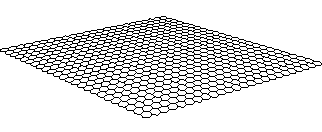
\includegraphics[width=\linewidth]{figures/torus-3d-flat.pdf}
				\caption{}
				\label{fig:torus-3d-flat}
			\end{subfigure}
			~~
			\begin{subfigure}{0.26\linewidth}
				\center
				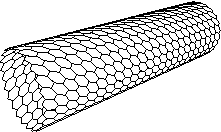
\includegraphics[width=\linewidth]{figures/torus-3d-tube.pdf}
				\caption{}
				\label{fig:torus-3d-tube}
			\end{subfigure}
			~~
			\begin{subfigure}{0.23\linewidth}
				\center
				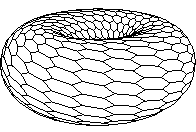
\includegraphics[width=\linewidth]{figures/torus-3d-torus.pdf}
				\caption{}
				\label{fig:torus-3d-torus}
			\end{subfigure}
			
			\caption{Visualisation of a hexagonal torus topology as a torus.}
			\label{fig:torus-3d}
		\end{figure}
		
		The wrap around connections in the topology are what give it the `torus'
		part of its name. Figure~\ref{fig:torus-3d-flat} shows a hexagonal torus
		topology drawn flat as in the previous figure. If the topology is rolled
		up into a tube such that the top and bottom chips become directly
		adjacent a tube is formed as in figure~\ref{fig:torus-3d-tube}. This tube
		can then be bent into a torus (i.e. doughnut) shape as in
		figure~\ref{fig:torus-3d-torus}, bringing together the chips at the ends
		of the tube.
		
		A hexagonal torus topology is typically defined in terms of its width and
		height along the X and Y axes respectively. For example,
		figure~\ref{fig:hexagonalTorusTopology} shows a $10\times10$ hexagonal
		torus.  The chips in a hexagonal torus topology are addressed using
		hexagonal coordinates of the form $(x, y, z)$ \cite{patel15}. The bottom
		left chip (labelled $\alpha$ in the figure) has the coordinate $(0, 0, 0)$
		and other chips are assigned coordinates according to the number of hops
		along each dimension they are from $(0, 0, 0)$, for example $\beta$ has the
		coordinate $(2, 0, -1)$.
		
		Counter intuitively, individual chips in hexagonal torus topologies may be
		described by many different coordinates, for example $(3, 1, 0)$ and $(1,
		-1, -2)$ are also a valid coordinates for $\beta$. These dual coordinates
		emerge from the fact that the vector $(1, 1, 1)$ results in no movement in
		a hexagonal torus topology. As a consequence, adding (or subtracting) this
		vector to any coordinate in a hexagonal topology results in an equivalent,
		but different, coordinate. This phenomenon is explored in greater detail in
		chapter \ref{sec:shortestPaths}.
		
		\begin{figure}
			\center
			\begin{subfigure}[b]{0.32\linewidth}
				\center
				\buildfig{figures/torus-compare-hexagonal.tex}
				
				\caption{Hexagonal}
				\label{fig:torus-compare-hexagonal}
			\end{subfigure}
			\begin{subfigure}[b]{0.32\linewidth}
				\center
				\buildfig{figures/torus-compare-2d.tex}
				
				\caption{2D}
				\label{fig:torus-compare-2d}
			\end{subfigure}
			\begin{subfigure}[b]{0.32\linewidth}
				\center
				\buildfig{figures/torus-compare-3d.tex}
				
				\caption{3D}
				\label{fig:torus-compare-3d}
			\end{subfigure}
			
			\caption{Visual comparison of torus topologies. In all figures, `wrap
			around' connections between nodes at the ends of each axis are omitted
			for clarity.}
			\label{fig:torus-compare}
		\end{figure}
		
		Despite its unusual coordinate system, hexagonal torus topologies compare
		favourably with more conventional network topologies such as 2D and 3D
		toruses (sometimes known as 2-ary $N$-cubes and 3-ary $N$-cubes
		respectively) \cite{dally04} illustrated in figure~\ref{fig:torus-compare}.
		Compared with a 2D torus topology, a hexagonal torus has double the
		bisection bandwidth even though it only requires 50\% more node-to-node
		links \cite{navaridas09}. Compared with 3D torus topologies, hexagonal
		torus topologies also have six node-to-node links per chip (i.e. the same
		network hardware is required) but only half the bisection bandwidth.
		However, since a network topology must eventually be embedded into a real
		world data centre (which at large scales approximates a 2D topology), 3D,
		or higher-dimensional torus topologies may become more expensive to
		construct in practice. As chapter \ref{sec:building} demonstrates,
		hexagonal toruses may be assembled in a machine room in a similar way to a
		2D topology. The hexagonal torus topology, therefore, presents an equally
		scalable but higher performance alternative to 2D toruses.
		
		\begin{figure}
			\center
			\begin{subfigure}[b]{0.45\linewidth}
				\center
				\buildfig{figures/hexagonal-torus.tex}
				\caption{Hexagonal torus}
				\label{fig:topo-compare-hexagonal-torus}
			\end{subfigure}
			\begin{subfigure}[b]{0.45\linewidth}
				\center
				\buildfig{figures/h-torus.tex}
				\caption{H-torus}
				\label{fig:topo-compare-h-torus}
			\end{subfigure}
			
			\caption{Hexagonal torus vs. H-torus topology. Each numbered hexagon
			represents a node. The thick outline indicates the bounds of the
			topology after which the network repeats. In each topology, the path
			taken by advancing in the Y$^+$ direction from the node labelled `0' is
			shown.}
			\label{fig:topo-compare}
		\end{figure}
		
		Confusingly, another family of network topologies called `H-torus'
		topologies have been defined, also composed of a hexagonal tiling of
		nodes arranged in a torus-like topology \cite{zhao08}. These topologies
		should not be confused with the hexagonal torus topology as defined in
		this chapter
		and used by SpiNNaker. H-torus topologies are more closely related to
		twisted torus topologies \cite{camara10} and as
		figure~\ref{fig:topo-compare} illustrates, have more complex 
	
	\section{Scaling-up SpiNNaker machines}
		
		\begin{figure}
			\center
			\begin{subfigure}[b]{0.45\linewidth}
				\center
				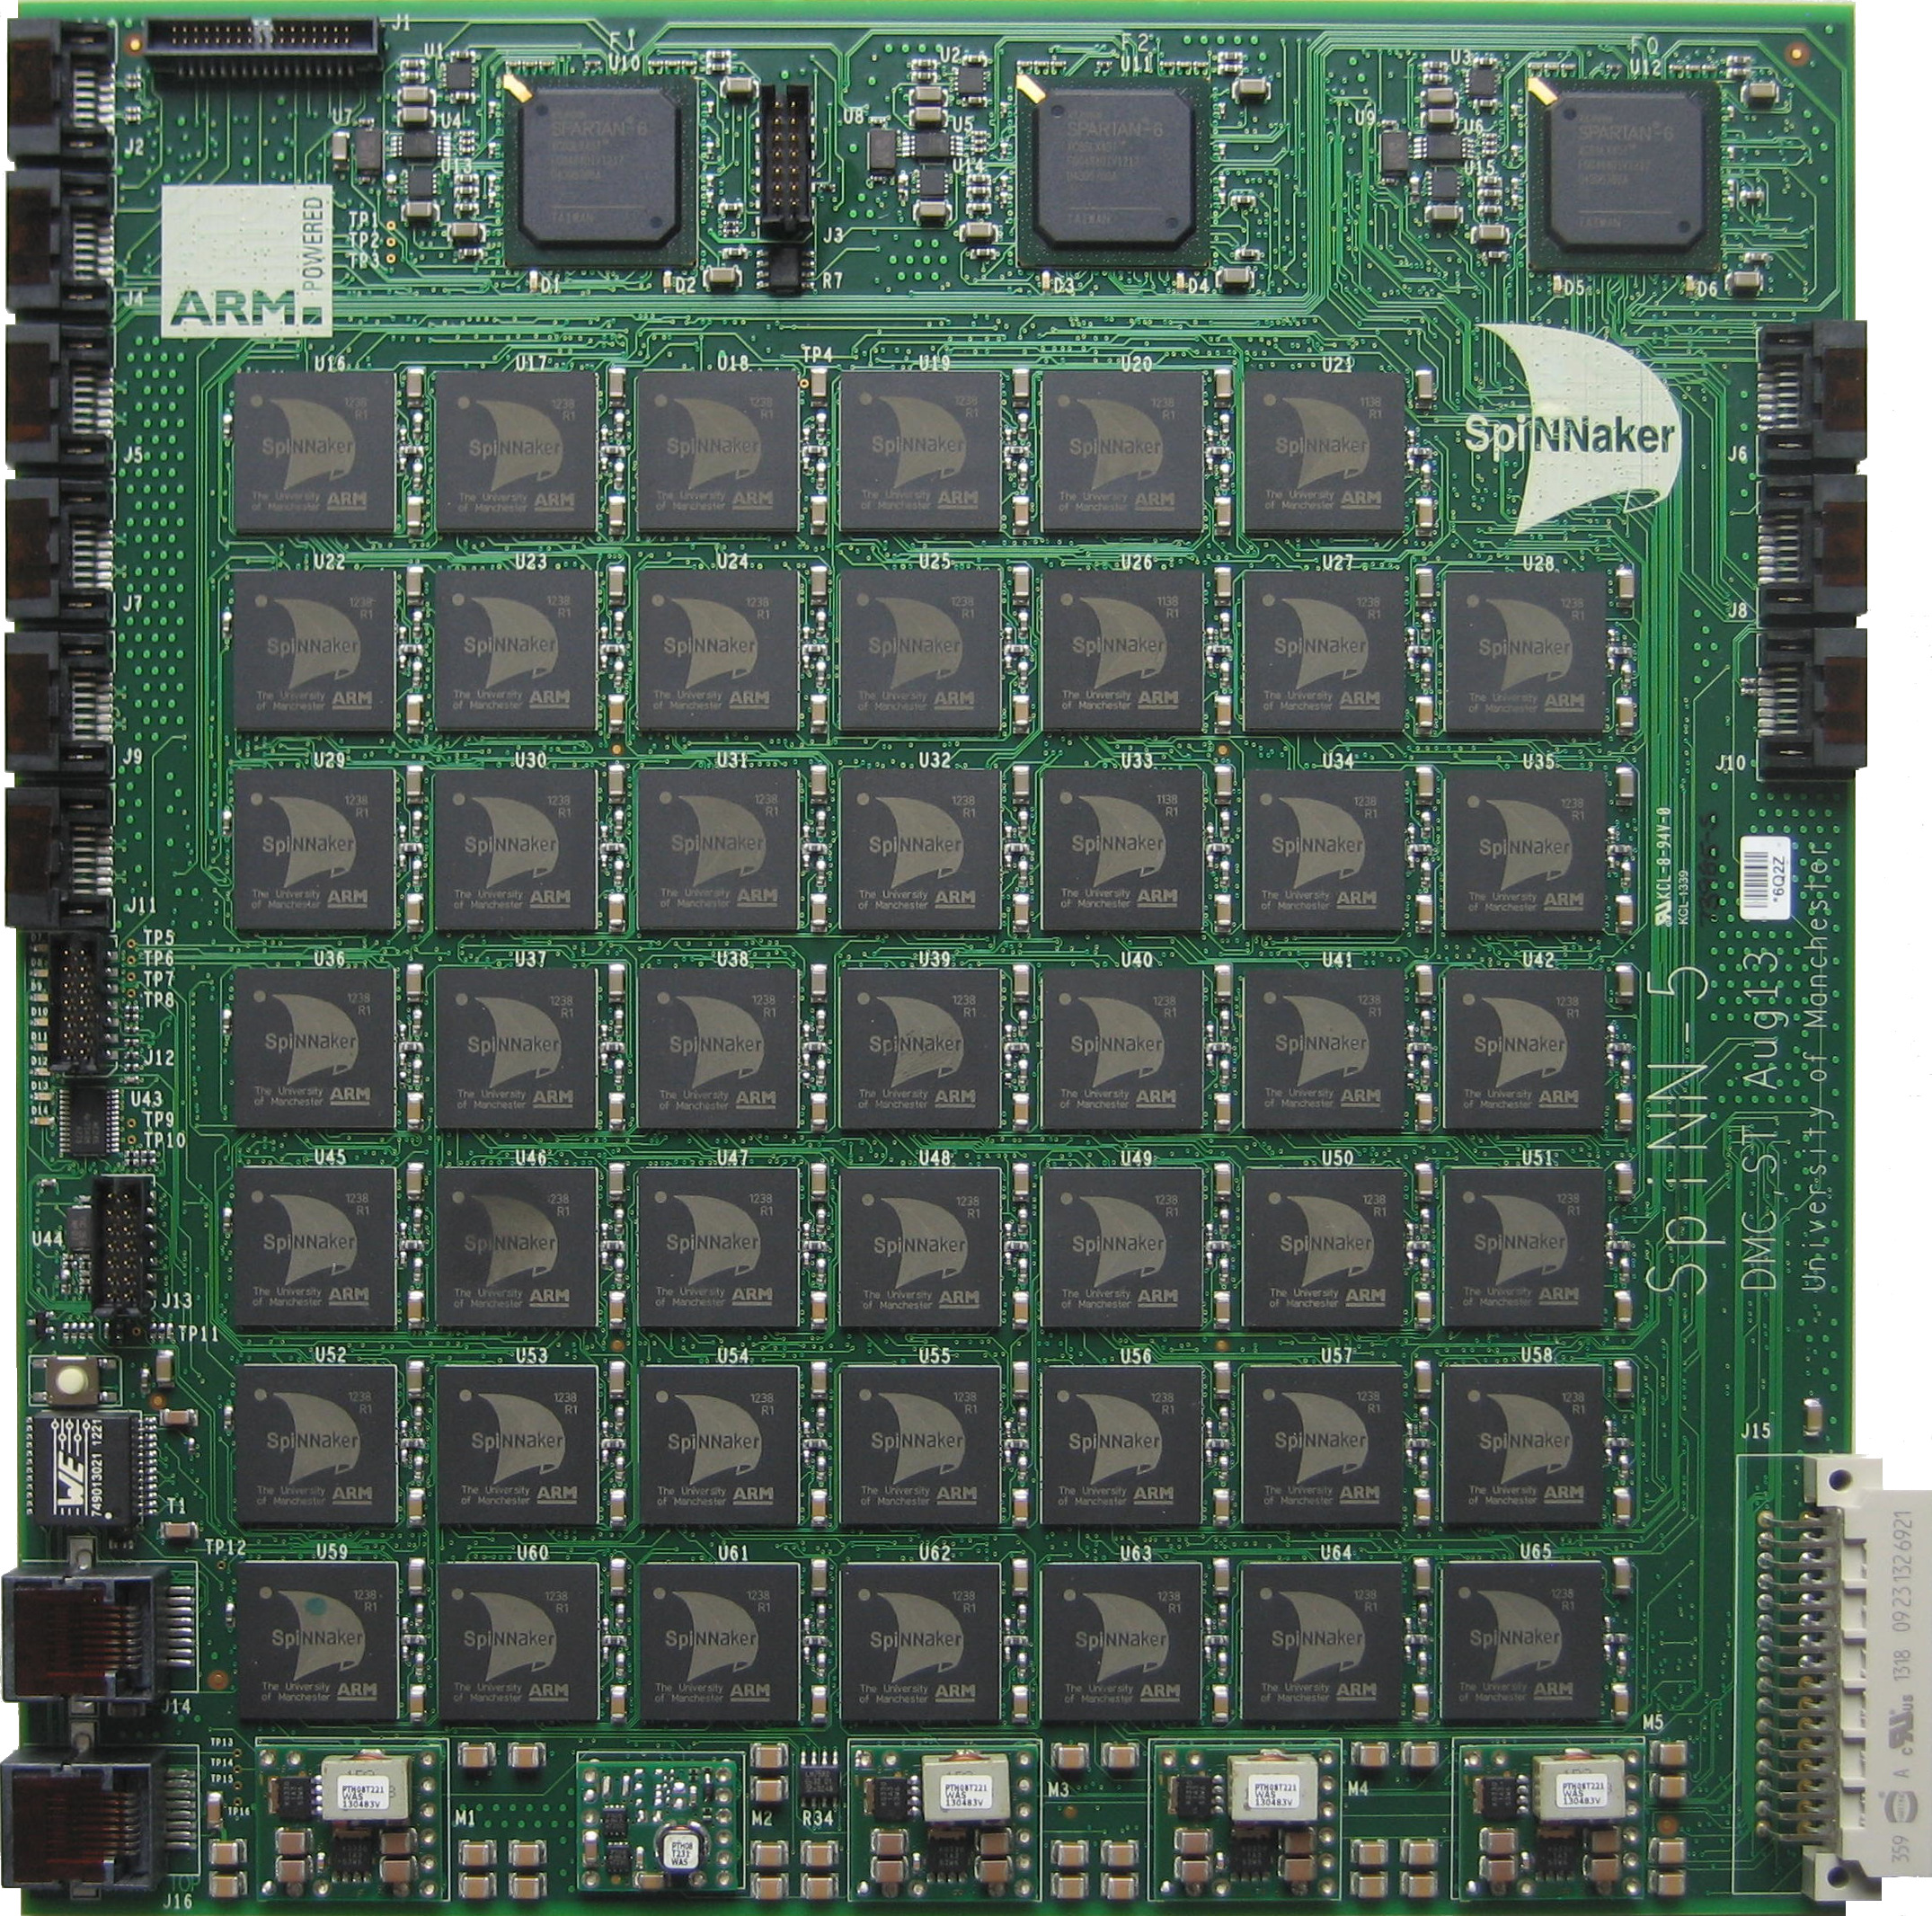
\includegraphics[width=\linewidth]{figures/spinnakerBoard.jpg}
				
				\caption{A SpiNNaker board}
				\label{fig:spinnakerBoard}
			\end{subfigure}
			~~~
			\begin{subfigure}[b]{0.45\linewidth}
				\center
				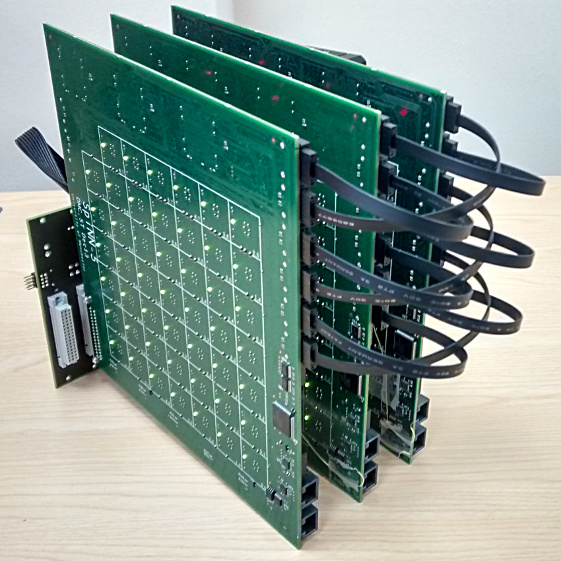
\includegraphics[width=\linewidth]{figures/threeboard.jpg}
				
				\caption{Three board system}
				\label{fig:threeboard}
			\end{subfigure}
			
			\vspace*{2em}
			
			\begin{subfigure}{\linewidth}
				\center
				\buildfig{figures/sata-connections.tex}
				
				\caption{The logical connectivity between chips in multi-board systems.
				Each board's forty-eight chips are arranged in a wrapped triple.
				Connections between chips on neighbouring boards are concentrated onto
				a single high-speed link.}
				\label{fig:sata-connections}
			\end{subfigure}
			
			\caption{SpiNNaker boards}
			\label{fig:spinnaker-boards}
		\end{figure}
		
		In order to build large SpiNNaker systems comprising tens of thousands of
		SpiNNaker chips, groups of forty-eight chips are mounted onto printed
		circuit boards as illustrated in figure~\ref{fig:spinnakerBoard}. These
		boards may be connected together to form larger systems.
		Figure~\ref{fig:threeboard} shows a prototype three board system configured
		as a $12\times12$ hexagonal torus topology.
		
		Though the chips are physically arranged in a (nearly) $7\times7$ grid on
		each SpiNNaker board, they logically form a `wrapped triple', a shape
		described in detail in appendix \ref{sec:partitioning} and shown in
		figure~\ref{fig:sata-connections}. Logically, the chips at the periphery of
		each board connect to their neighbours on the six adjacent boards.
		Normally SpiNNaker chips use a low power, asynchronous 2-of-7 protocol
		requiring sixteen wires per bidirectional chip-to-chip link
		\cite{bainbridge03}. If this link technology were used to connect chips on
		neighbouring boards, each neighbouring would need to be connected by a
		128~wire cable. Cables and connectors supporting this may signals are
		expensive and physically large making them unsuitable for use with
		SpiNNaker. Instead, all chip-to-chip connections to the same board are
		multiplexed and demultiplexed onto a single high-speed serial link
		\cite{athavale05} carried via commodity S-ATA cables (often used to
		connected hard disks in desktop computers and servers) \cite{sata3spec}.
		The six high-speed links are implemented by three onboard FPGAs (the three
		large chips at the top of the SpiNNaker board) and are logically
		transparent to the underlying network.
		
		In chapter~\ref{sec:building} I describe how very large SpiNNaker machines
		may be constructed using over one thousand SpiNNaker boards.
